\documentclass[12pt]{article}
\usepackage[utf8]{inputenc}
\usepackage{graphicx}
\usepackage{fixltx2e}
\graphicspath{{images/}}
\title{Rendszer- és irányításelmélet esti 2017-18 tavasz házi feladat}
\author{Benkő Gábor}
\date{\today}
\begin{document}
\maketitle
\newpage
\section{Empirikus szabályozótervezés}
\subsection{Szabályozó tervezés Ziegler-Nichols kísérleti identifikáción alapuló szabályozás módszerével}
\begin{figure}[h]
    \centering
	\includegraphics[scale=.4]{stepresponse}
	\caption{A szabályozandó rendszer ugrásválasza}
	\label{fig:stepresponse}
\end{figure}
Az ábrán látható megadott ugrásválasz alapján kerül tervezésre a PID szabályozó. Az ugrásválasz alapján az identifikáció alapján az alábbi értékek kerültek kinyerésre:
\begin{center}
\begin{tabular}{|c c c|}
\hline Név & Jelölés & Érték \\
\hline \hline
Holtidő & T\textsubscript{u} & 4\textsubscript{s} \\
\hline
Felfutási idő & T\textsubscript{r} & 12\textsubscript{s} \\
\hline
A szakasz erősítése & K\textsubscript{p} & 4 \\
\hline
\end{tabular}
\end{center}
Az eredményekből kiszámolásra került a $\rho=\frac{T_u}{T_r}=\frac{4}{13}=0.3333$ értéke, illetve a $T_I=2*T_U=8$ és a $T_D=T_U=4$. Az $A_p$ értéke kiszámolása a $A_p*K_p*\rho\leq1.2$ egyenlet átrendezésével \[A_P\leq\frac{1.2}{K_P*\rho}\leq0.9000\]
A PID szabályozó átviteli függvénye \[W\textsubscript{PID}=0.9000*(1+\frac{1}{8s}+4s)\]
ahol a MATLAB alapján keletkezett átviteli függvény \[W\textsubscript{PID}=\frac{3.6s^2+0.9s+0.1125}{s}\].
A Simulink-ban létrehozott rendszer ugrásválasza:
\begin{figure}[h]
\centering
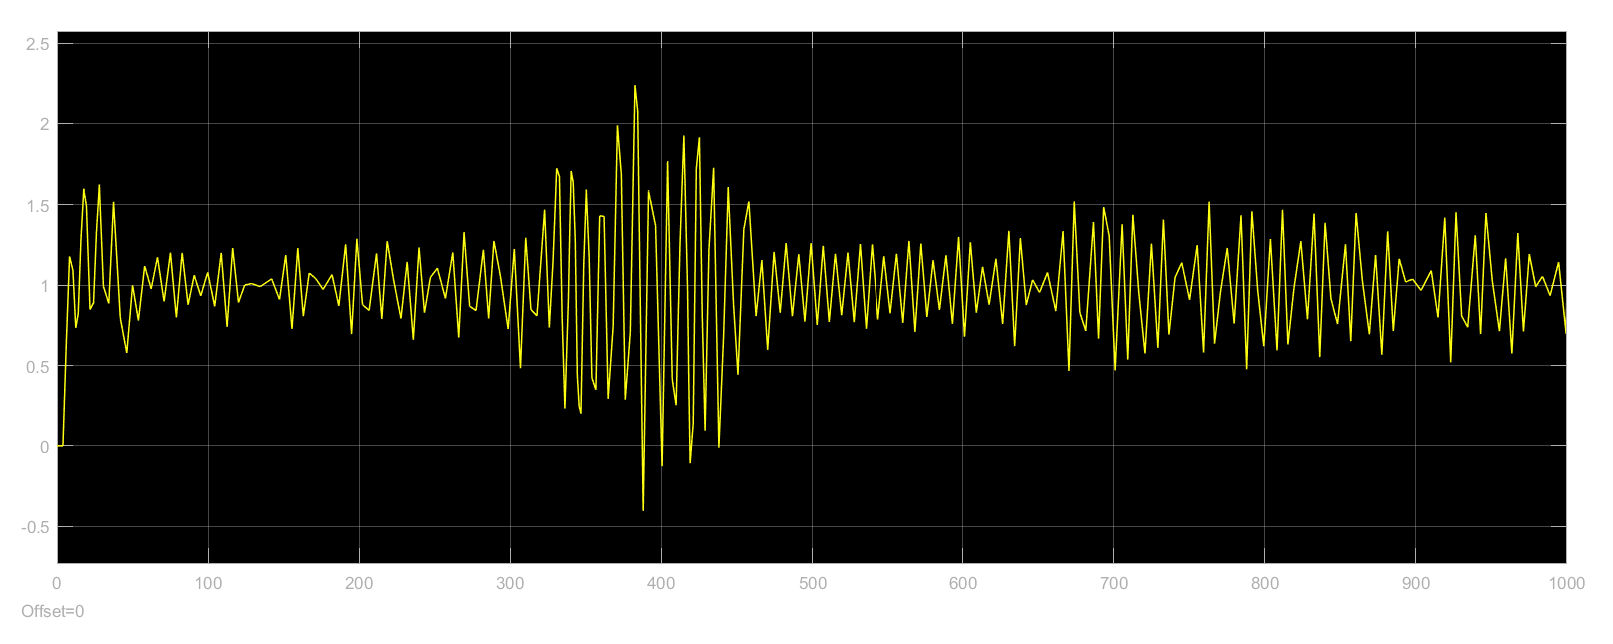
\includegraphics[scale=.50]{zgpidosc}
\caption{Az $A_P=0.9000$ rendszer ugrásválasza}
\end{figure}
Az ugrásválasz alapján látható a rendszer a stabilitás határán van. Ha rendszer stabilan szeretnénk tartani akkor $A_P<0.9000$ kell lennie. Így empirikus módszer segítségével csökkentjük az erősítési tényezőt, amíg megtaláljuk a közeli erősítési tényezőt.
A felezési módszertannal $A_P=0.1000$ esetén:
\newpage
\begin{figure}[h]
\centering
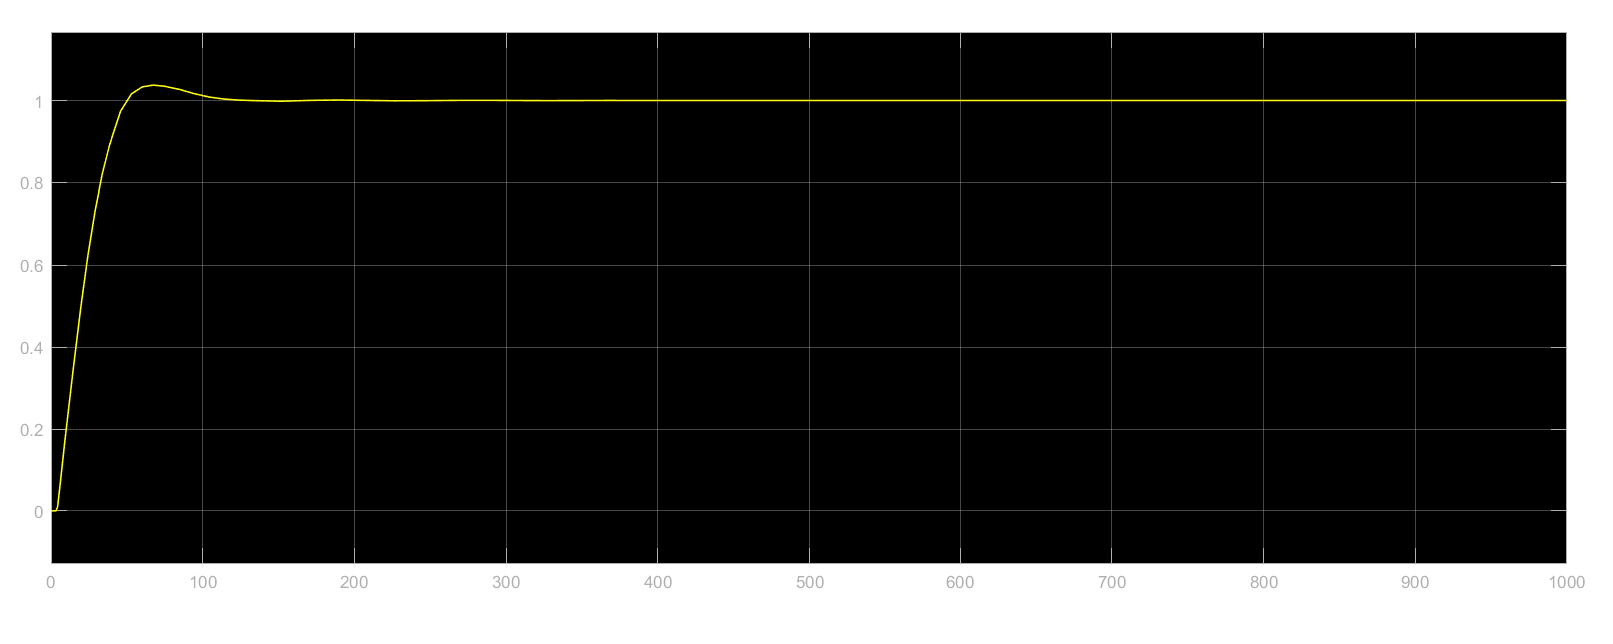
\includegraphics[scale=.50]{ap0100}
\caption{Az $A_P=0.1000$ rendszer ugrásválasza}
\end{figure}
a rendszerünk már stabil, illetve van egy kis túllövése, mely után beáll állandósult állapotba. A rendszer erősítését így tovább növelhetjük. A felezési módszer alapján, most az $A_P=0.4500$ erősítés esetén:
\newpage
\begin{figure}[h]
\centering
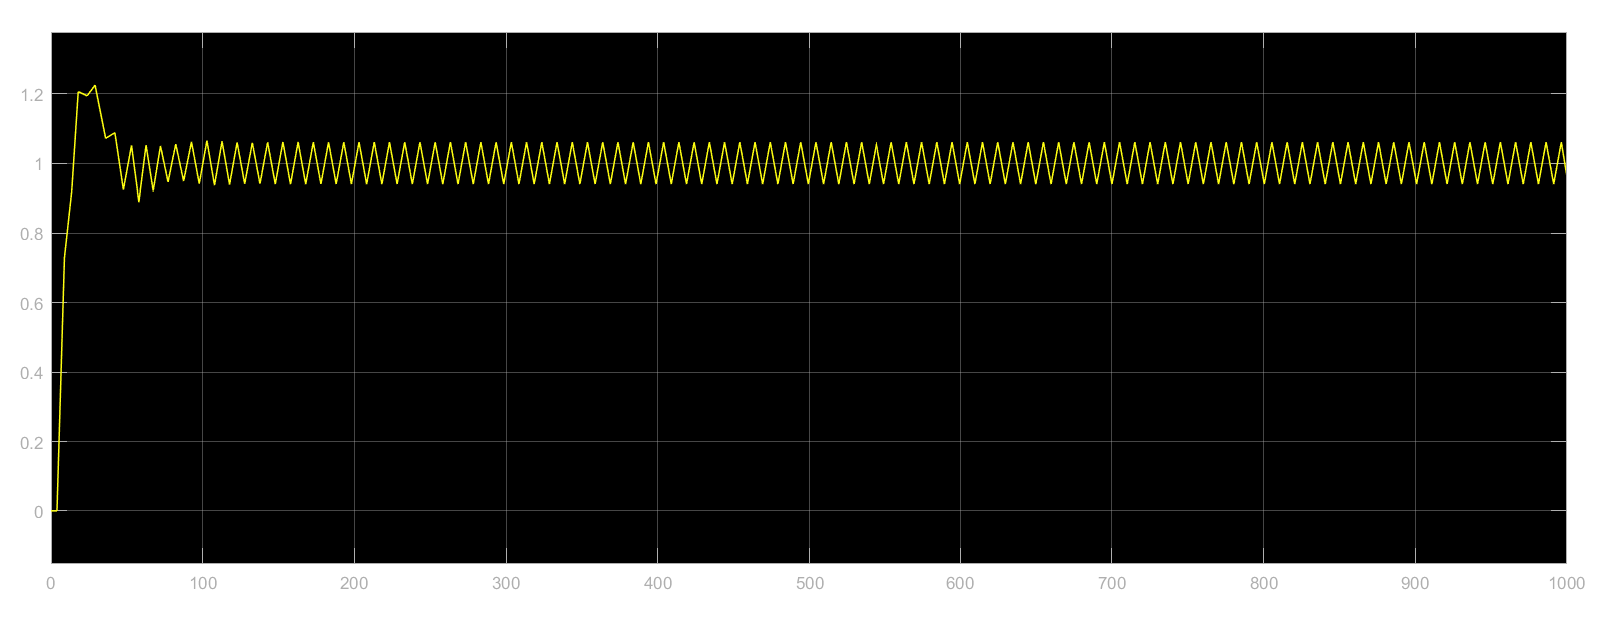
\includegraphics[scale=.50]{ap0450}
\caption{Az $A_P=0.4500$ rendszer ugrásválasza}
\end{figure}
A rendszer most a stabilitás határán van, így az erősítés tényezőt csökkentem $A_P=0.225$ értékre.
\newpage
\begin{figure}[h]
\centering
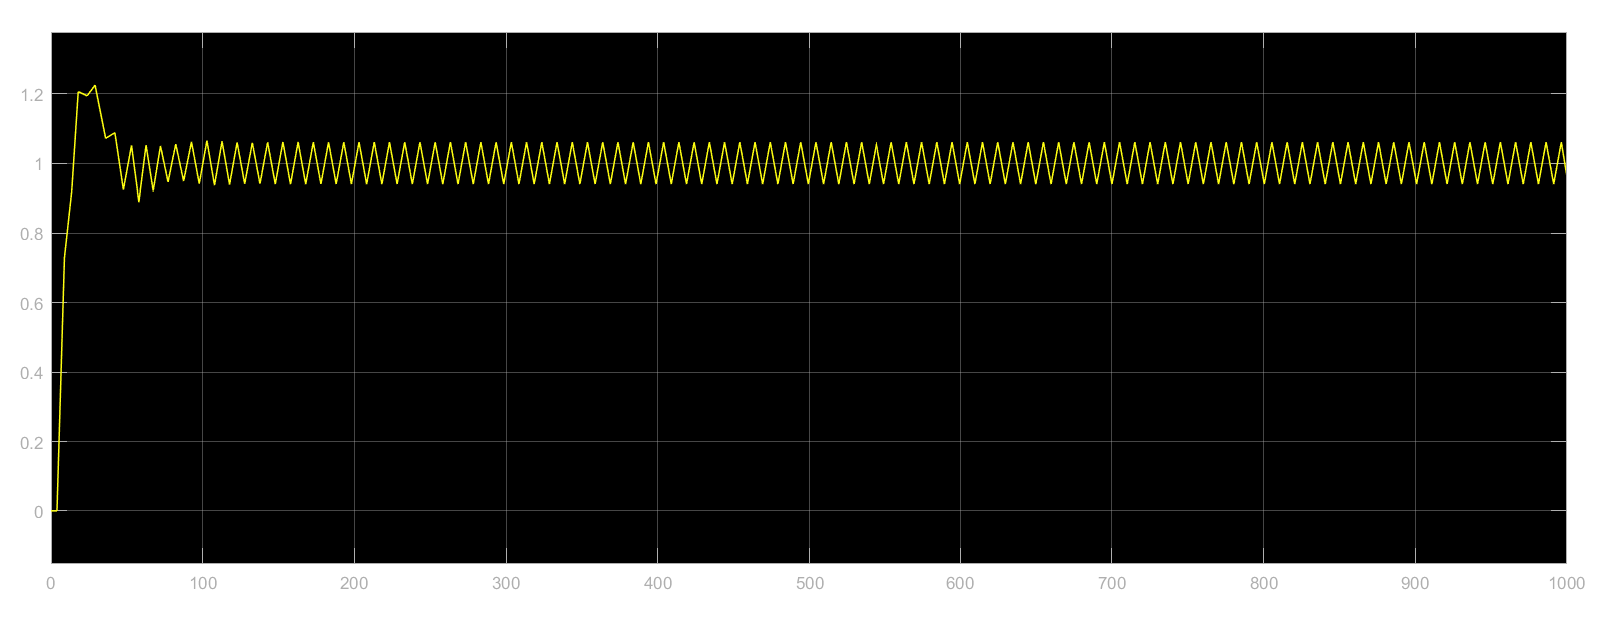
\includegraphics[scale=.50]{ap0450}
\caption{Az $A_P=0.2250$ rendszer ugrásválasza}
\end{figure}
A rendszer $A_P=0.2250$ estén stabil és van túllövése. Az $A_P$ értéke növelhető $A_P=0.337$.
\newpage
\begin{figure}[h]
\centering
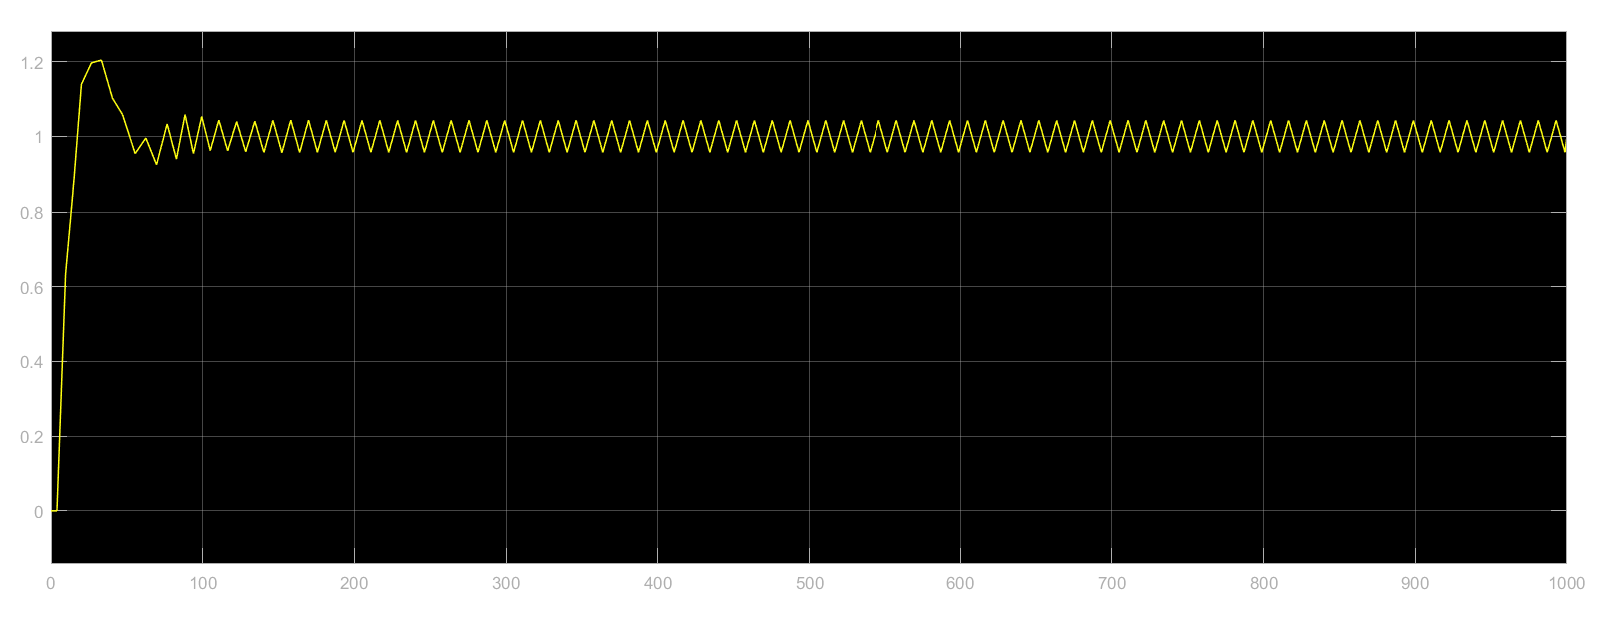
\includegraphics[scale=.50]{ap337}
\caption{Az $A_P=0.3370$ rendszer ugrásválasza}
\end{figure}
A rendszer a stabilitás határán van, így az $A_P=0.2810$ értékre csökkentve az ugrásválasz:
\newpage
\begin{figure}[h]
\centering
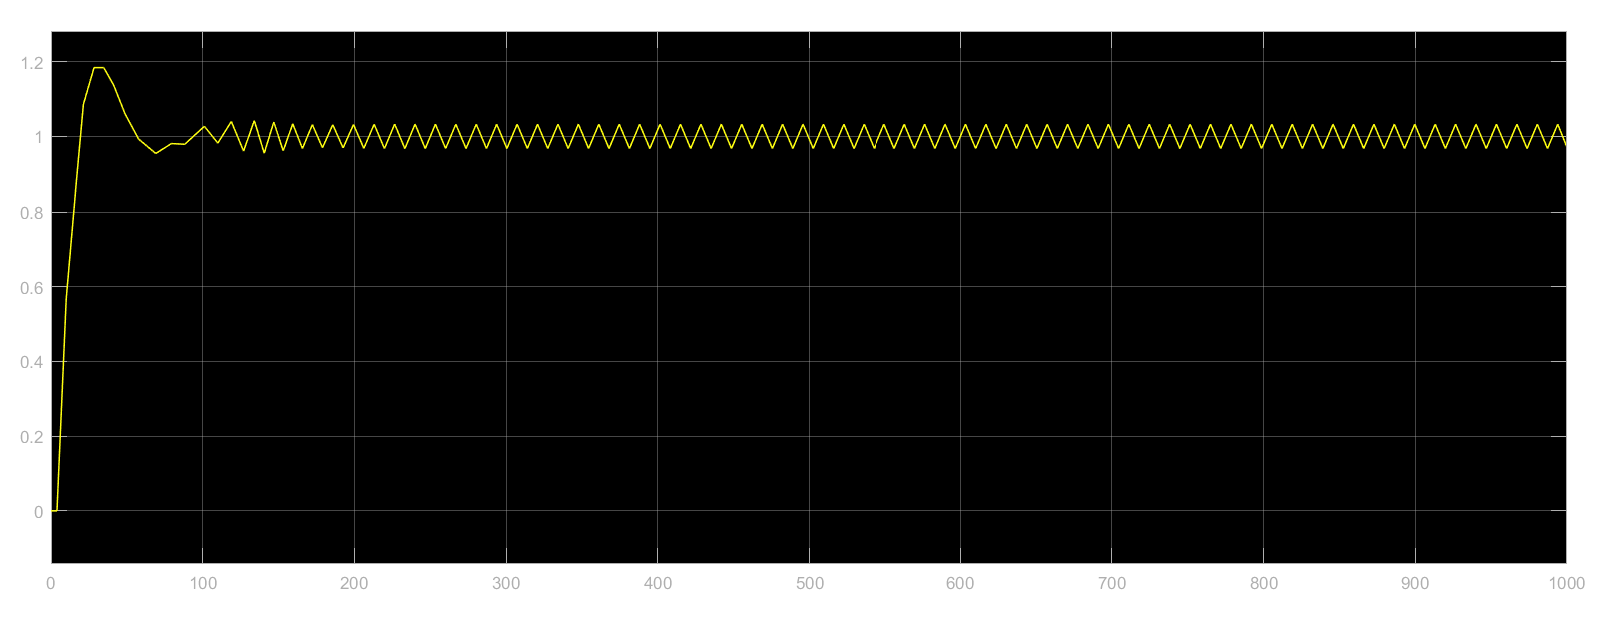
\includegraphics[scale=.50]{ap02810}
\caption{Az $A_P=0.2810$ rendszer ugrásválasza}
\end{figure}
A rendszer a stabilitás határán van továbbra is, így az $A_P$ értékét $A_P=0,2530$-ra csökkentem.
\newpage
\begin{figure}[h]
\centering
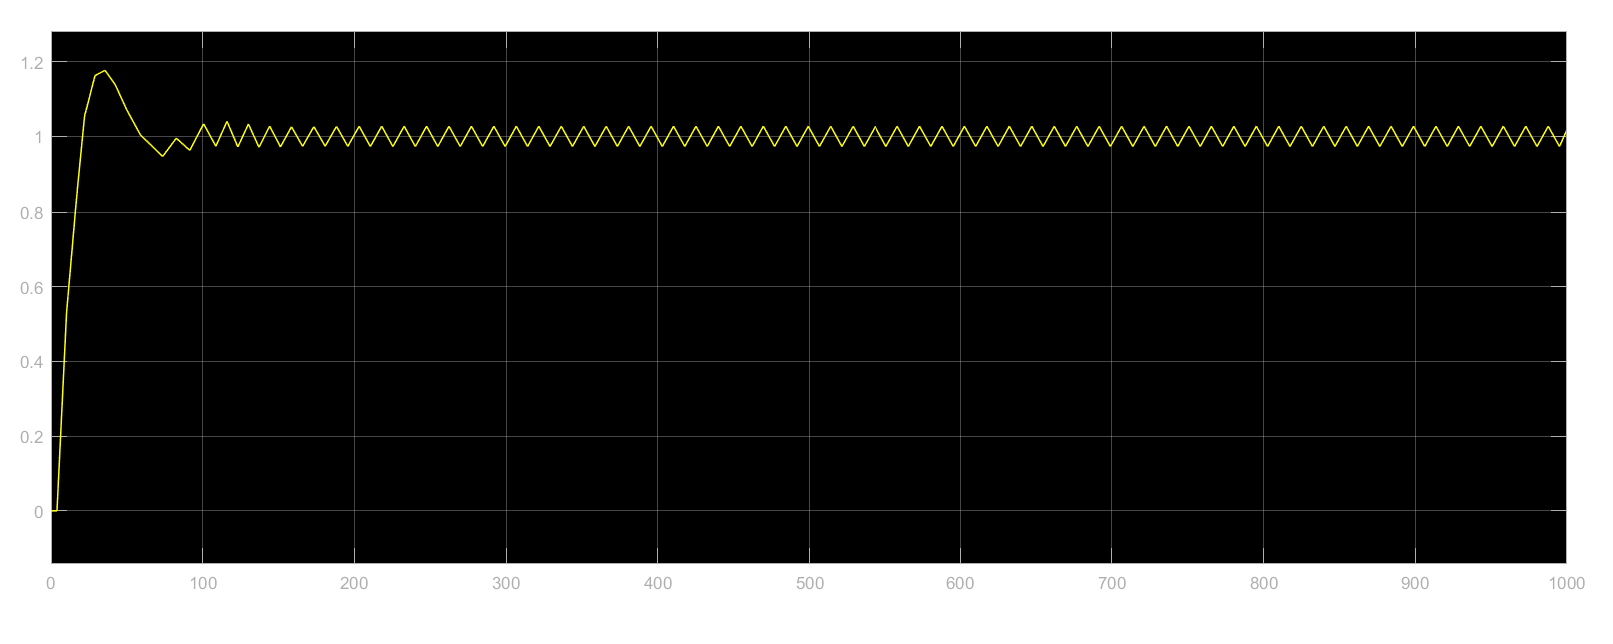
\includegraphics[scale=.50]{ap0253}
\caption{Az $A_P=0.2530$ rendszer ugrásválasza}
\end{figure}
A rendszer továbbra is stabilitás az határán, így az $A_P$ értékét $A_P=0.2390$-re csökkentem.
\newpage
\begin{figure}[h]
\centering
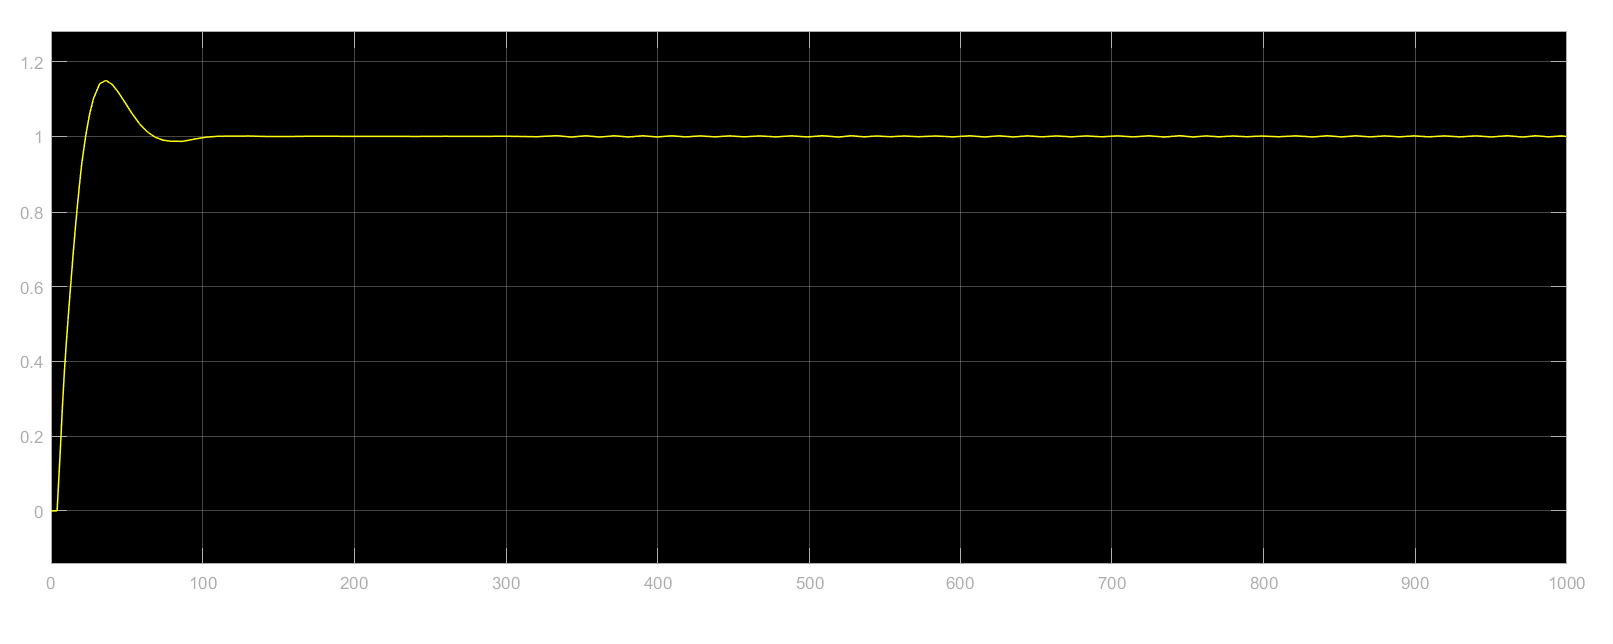
\includegraphics[scale=.50]{ap0239}
\caption{Az $A_P=0.2390$ rendszer ugrásválasza}
\end{figure}
A rendszer stabil így az $AP_P$ értékét $A_P=0.2460$-re növelem.
\newpage
\begin{figure}[h]
\centering
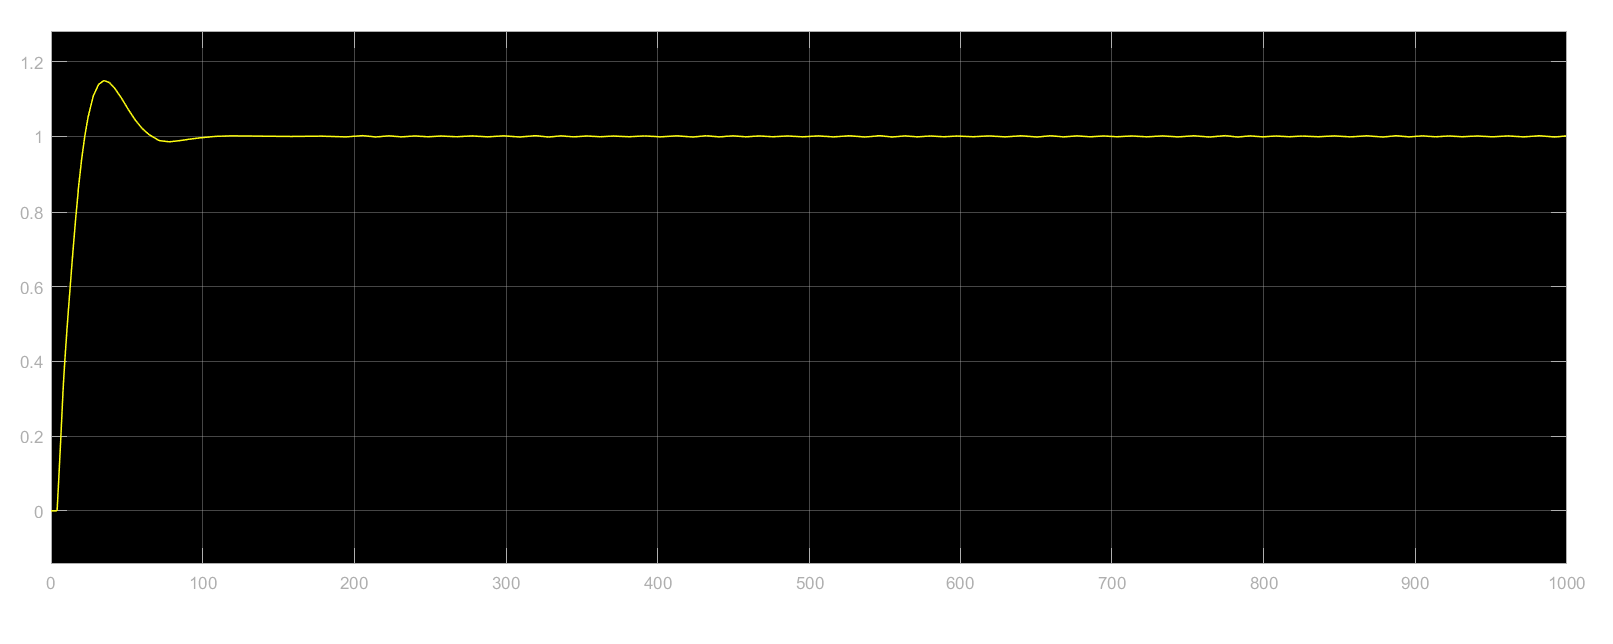
\includegraphics[scale=.50]{ap0246}
\caption{Az $A_P=0.2460$ rendszer ugrásválasza}
\end{figure}
A rendszer stabil így az $A_P$ értékét $A_P=0,2500$-re növelem.
\newpage
\begin{figure}[h]
\centering
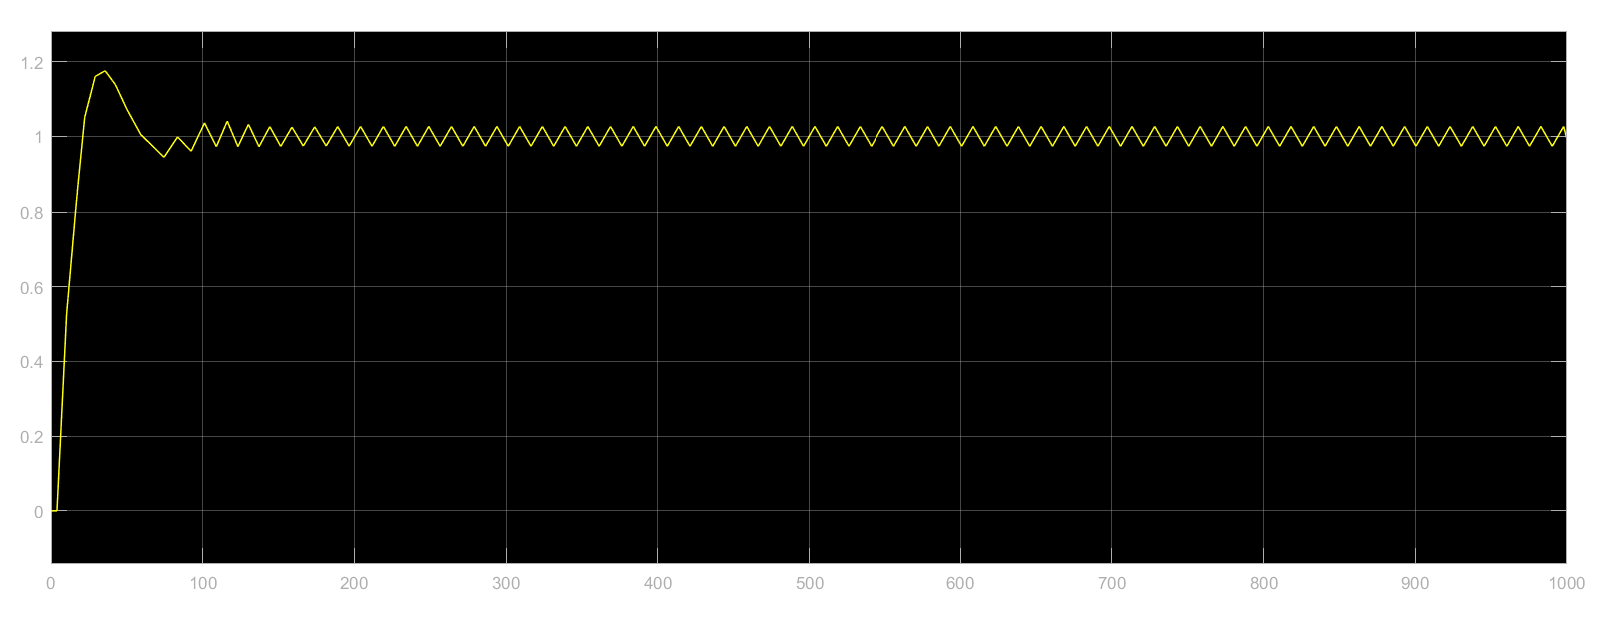
\includegraphics[scale=.50]{ap02500}
\caption{Az $A_P=0.2500$ rendszer ugrásválasza}
\end{figure}
A rendszer a stabilitás határán van, így az $A_P$ értékét $A_P=2482$-re csökkentem.
\newpage
\begin{figure}[h]
\centering
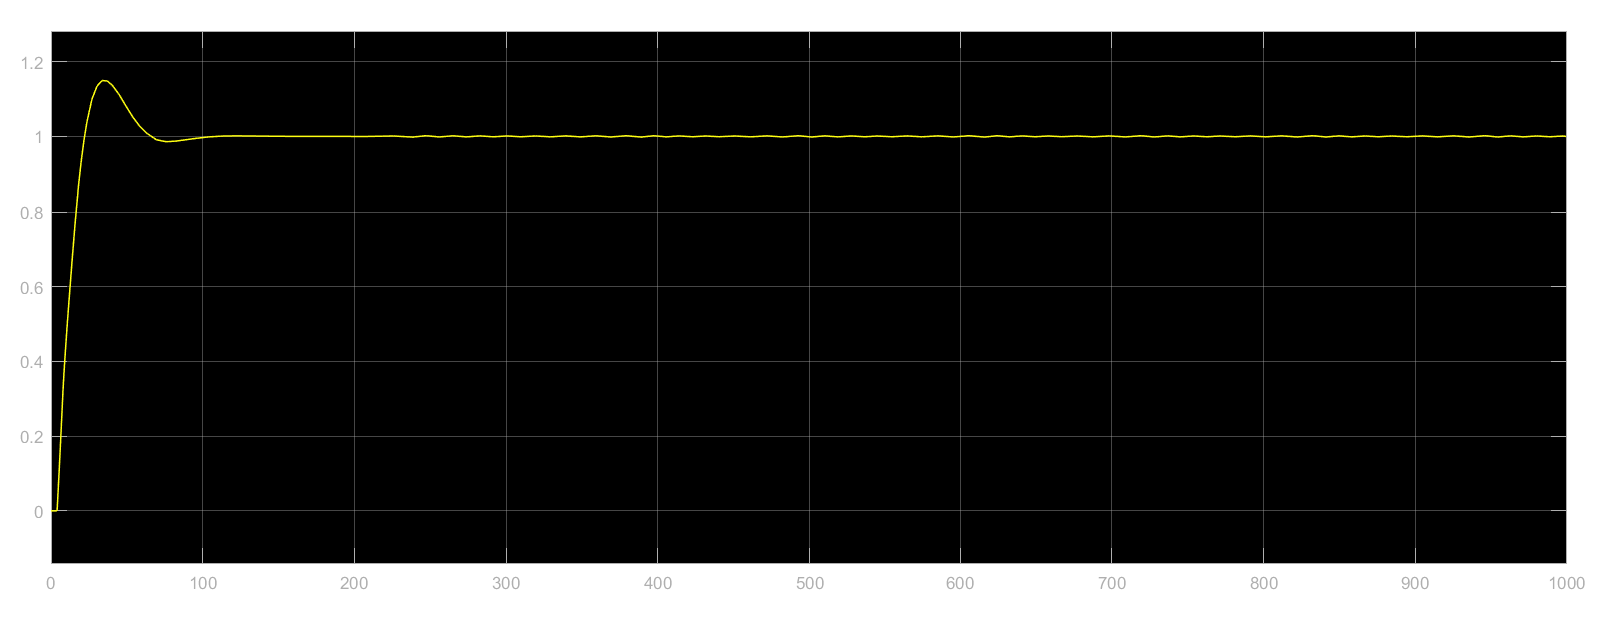
\includegraphics[scale=.50]{ap02482}
\caption{Az $A_P=0.2482$ rendszer ugrásválasza}
\end{figure}
A rendszer stabil, így 3 tizedesjegy pontosságra térve, az $A_P$ erősítést $A_P=.0249$ értékre növeltem, mivel látható, hogy $A_P=0.250$ estén már a stabilitás határán van a rendszer.
\newpage
\begin{figure}[h]
\centering
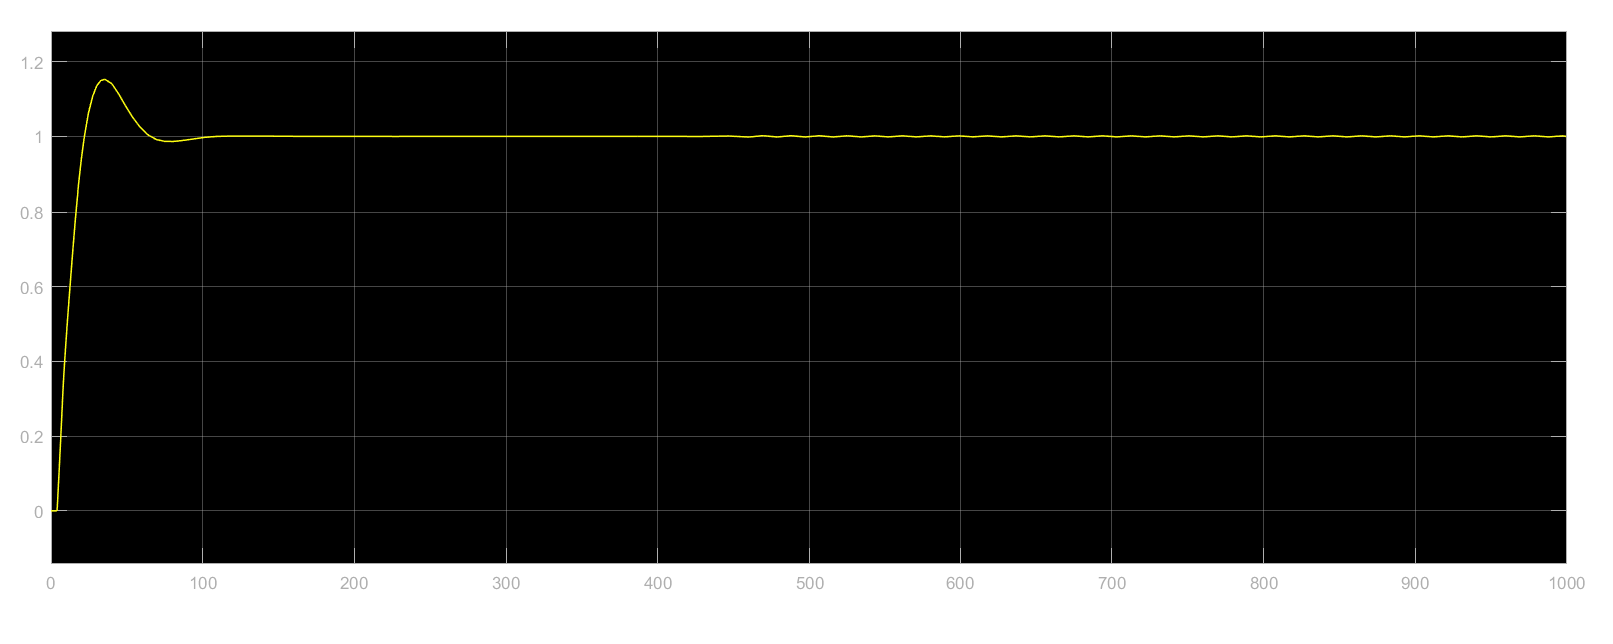
\includegraphics[scale=.50]{ap0249}
\caption{Az $A_P=0.249$ rendszer ugrásválasza}
\end{figure}
A rendszer stabil, van egy túllövése, majd egy alul lövést követve beáll a rendszer állandósult állapotba. A mérések alapján kijelenthető, hogy $A_P=0.249$ erősítésig lehet a rendszert erősíteni.

\end{document}